
%
% Computational Astrophysics
%

\documentclass{article}

%-------------------------------------------------------------------------------------------------------------
%  package
%--------------------------------------------------------------------------------------------------------------
%版面規劃(a4大小,上下左右距0.9inch)
\usepackage[a4paper,margin=0.9in]{geometry}

%和插入圖片相關的package
\usepackage{graphicx}
\usepackage[FIGTOPCAP]{subfigure}

\usepackage{amsmath,booktabs,threeparttable,url, bm}
%\usepackage[hyphenbreaks]{breakurl}

%連結註腳網頁
\usepackage[colorlinks,linkcolor=blue]{hyperref}

%中文化package
\usepackage{CJKutf8}

%\newcommand{\cntext}{\begin{CJK}{UTF8}{bsmi}\end{CJK}}

\title{Assignment 2 of Computational Astrophysics in NTHU}
\author{Wei-Hsiang Yu 游惟翔}


%-------------------------------------------------------------------------------------------------------------
%  文件開始
%--------------------------------------------------------------------------------------------------------------
\begin{document}

\begin{CJK}{UTF8}{bsmi}
%中文化需要加上此行才有title/author/date
\maketitle
\end{CJK}


%-------------------------------------------------------------------------------------------------------------
%  Written Assignments
%--------------------------------------------------------------------------------------------------------------
\section{Written Assignments}

%Q1---------------------------------------------------------------------
\underline{\textbf{Q1 : Derive the Kepler’s Law\\}}

\textbf{Kepler’s Second Law}
\begin{equation}
    A = \frac{1}{2}\frac{L}{\mu}P
    \label{eq:k2}
\end{equation}

Where $A=\pi ab$ is the area of ellipse, $L$ is angular momentum, $\mu$ is reduced mass, $P$ is orbital period.

$<pf> :$

In polar coordinates,
\begin{equation}
    \vec{r} = r\hat{r} = r(\hat{i}\cos{\theta}+\hat{j}\sin{\theta})
    \label{eq:k2_r}
\end{equation}

Derivatives Eq.\ref{eq:k2_r}. with respect to time $t$,
\begin{equation}
    \frac{d\vec{r}}{dt} = \frac{dr}{dt}(\hat{i}\cos{\theta}+\hat{j}\sin{\theta}) 
    + r(-\hat{i}\sin{\theta}\frac{\theta}{dt}+\hat{j}\cos{\theta}\frac{\theta}{dt})
    =\dot{r}\hat{r}+r\omega\hat{\theta}
    \label{eq:k2_r'}
\end{equation}

So the area swept by $\vec{r}$ during time $dt$ is (Fig..) :
\begin{equation}
    dA = \frac{1}{2}\left|\vec{r}\times\vec{v}\right|
    = \frac{1}{2}\left|r\hat{r}\times(\dot{r}\hat{r}+r\omega\hat{\theta})\right|
    = \frac{1}{2}r^2\omega dt
    \label{eq:k2_a}
\end{equation}

and we eliminate Eq.\ref{eq:k2_a}. to get :
\begin{equation*}
    \frac{dA}{dt} = \frac{1}{2}r^2\omega
    \label{eq:k2_a'}
\end{equation*}

Recall that $L=\vec{r}\times\vec{p}=\mu r^2\omega$, so we substitute and get Kepler’s Second Law \\
(Here, angular momentum is produced by $m_1$ \& $m_2$ relative to center of mass, so we use reduced mass $\mu$)

$$A = \frac{1}{2}\frac{L}{\mu}P$$

%克普勒3--------------------------------------------------------------
\textbf{Kepler’s Third Law}
\begin{equation}
    P^2 = \frac{4\pi^2}{G(m_1+m_2)}a^3
    \label{eq:k3}
\end{equation}

Where $a$ is the binary separation, and $m_1$ and $m_2$ are masses.

$<pf> :$

By center of mass, we can say that :
\begin{equation*}
    m_1a_1=m_2a_2
    \label{eq:k3_center}
\end{equation*}

and we can make $a_1=\frac{m_2a_2}{m_1}$,so we will have Eq.\ref{eq:k3_a}.

\begin{equation}
    a=(\frac{m_2+m_1}{m_1})a_2
    \label{eq:k3_a}
\end{equation}

We can see Fig.., $m_2$ has two force act on it : gravity \& centripetal acceleration.
They should be equal!
\begin{equation}
    F_{gravity}=\frac{Gm_1m_2}{a^2}=F_{centripetal}=m_2a_2{\omega}^2
    \label{eq:k3_equal}
\end{equation}

Then, we substitute the binary separation $a$(Eq.\ref{eq:k3_a}.) to Eq.\ref{eq:k3_equal}. and replace $\omega=\frac{2\pi}{P}$

$$\frac{Gm_1m_2}{a^2}
=\frac{m_1m_2}{m_1+m_2}a(\frac{2\pi}{P})^2$$

After eliminating, we can get Kepler's Third Law

$$P^2 = \frac{4\pi^2}{G(m_1+m_2)}a^3$$


%-------------------------------------------------------------------------------------------------------------
%  Programming Assignments
%--------------------------------------------------------------------------------------------------------------
\section{Programming Assignments}

%Q1---------------------------------------------------------------------
\underline{\textbf{Q1 : Sun-Earth system.\\}}
%-------------------------------
\begin{figure}[h]
    \centering 
	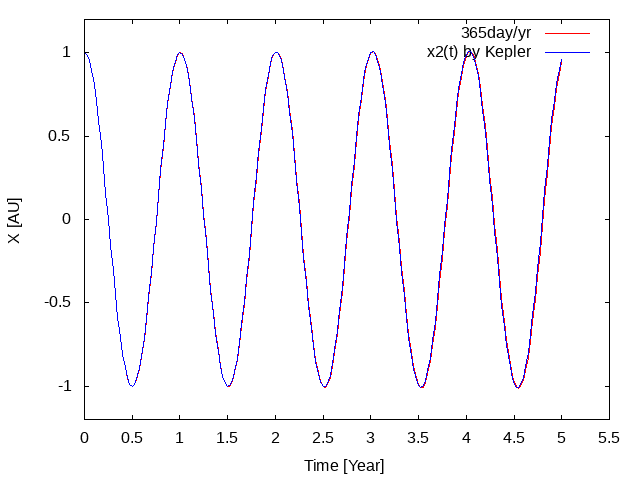
\includegraphics[scale=0.45]{pro1_x2.png}
	\caption{The trajectory of $m_1$ $m_2$ (when $m_2$ has a 1.25 factor of velocity).} %圖片註解
	\label{fig.pro1} %label 用這個就可以引用文章當中
\end{figure}
%-------------------------------

The blue line is my computed result used by Kepler's Third Law.
The red line uses 365 days as 1 year to run program.
In Fig.\ref{fig.pro1}., we can say that it's not very obvious different by using two different period.
But we can see the line's trough to the x axis, the fifth trough doesn't match in time=4.5yr as the first trough does in time=0.5yr.\\ \\
%Q2---------------------------------------------------------------------
\underline{\textbf{Q2 : Consider more \& some different perturbation}}

\textbf{2a.}

%-------------------------------
\begin{figure}[h]
    \centering 
	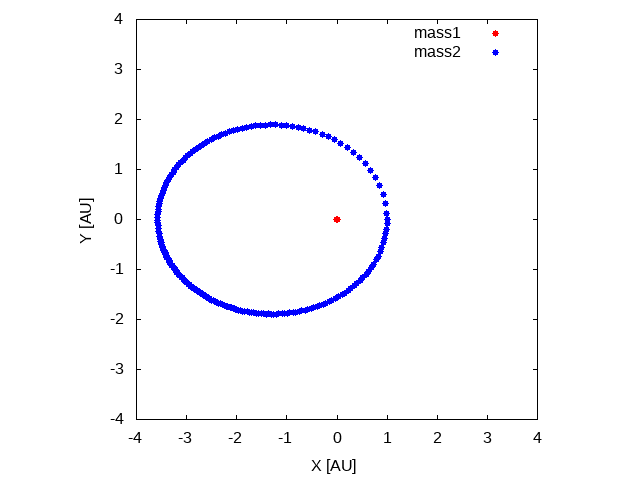
\includegraphics[scale=0.5]{pro2_a.png}
	\caption{The trajectory of $m_1$ $m_2$ (when $m_2$ has a 1.25 factor of velocity).} %圖片註解
	\label{fig:pro2_a} %label 用這個就可以引用文章當中
\end{figure}
%-------------------------------


\textbf{2b.Perihelion and Aphelion}\\
As the question say, we know that:
\begin{equation}
r_p=a(1-e)=1au
\label{eq:2b}
\end{equation}

$r_p$ , the position of the perihelion, will be $1au$ , which is the initial condition we give to the program.

Later, we need to find the position of mass2 at the aphelion in order to acquire "a" in Eq.\ref{eq:2b}. We find the file[binary002.dat] to get the the closet two position to aphelion:

$$x_2=-0.534935585707E+14  \qquad  y_2=-0.211156452869E+12$$
$$x_1=-0.534872149361E+14  \qquad  y_1=0.609624905270E+12$$

So after using interpolation, we can get the position of aphelion (at y=0) is $-0.5349192658994514E+14$, and substitute it to Eq.\ref{eq:2b}. and get the eccentricity $e=0.562909......$

\begin{equation}
Velocity\ at\ Perihelion \qquad v^2= \frac{GM_\odot}{a} \frac{1+e}{1-e}
\label{eq:2b_+}
\end{equation}

\begin{equation}
Velocity\ at\ Aphelion \qquad v^2= \frac{GM_\odot}{a} \frac{1-e}{1+e}
\label{eq:2b_-}
\end{equation}

%-------------------------------
\begin{figure}[h]
    \centering 
	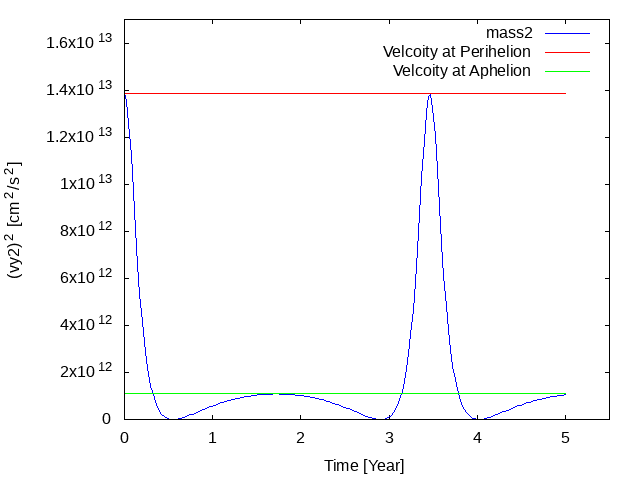
\includegraphics[scale=0.45]{pro2_b.png}
	\caption{${v_{y,2}}^2(t)$ and the velocity at Perihelion and Aphelion.} %圖片註解
	\label{fig:pro2_b} %label 用這個就可以引用文章當中
\end{figure}
%-------------------------------

We can see that in Fig.\ref{fig:pro2_b}. star will move rapidly when it is closed to Perihelion (blue line is sharp) and will move slowly when it is closed to Aphelion (blue line become smooth).\\

\textbf{2c.Conservation of $L(t)$ and  $E(t)$}\\
We know that the angular momentum is
\begin{equation}
L= \vec{r} \times \vec{p}
\label{eq:2c_l}
\end{equation}
and in our program we use orthogonal coordinates to analyze binary system.

So we already have $\vec{r_x}$,$\vec{r_y}$,$\vec{v_x}$,$\vec{v_x}$ and substitute into Eq.\ref{eq:2c_l}.

$$L=(\vec{r_x}+\vec{r_y}) \times m(\vec{v_x}+\vec{v_x})=m(r_xv_y-r_yv_x)$$

About energy, there is a equation
\footnote{the total energy in the binary system, page24-28 :
\href{https://web.njit.edu/~cao/hw4.pdf}{https://web.njit.edu/~cao/hw4.pdf}}
can calculate the total energy in the binary system,

\begin{equation}
E = K + U=\frac{1}{2}m{\frac{GMm}{L}}^2(e^2-1)
\label{eq:2c_e}
\end{equation}

So I put this two equation into [output.f90] and modify some format of the output file.
Remember that Eq.\ref{eq:2c_l}. only get mass1 or mass2 independently, the total angular momentum will be $L_{m1}+L_{m2}$. However, Eq.\ref{eq:2c_e}. represent the whole system.

\textbf{The result is there are both "closed" to conservation!}
There are closed because the order of the value are all the same, but still have error. Furthermore, the error will also pass to the next step, and a larger time step will has larger error in the same step.(see Fig.\ref{fig:2c_dat}.)

% %-------------------------------
% \begin{figure}[h]
%     % \centering 
% 	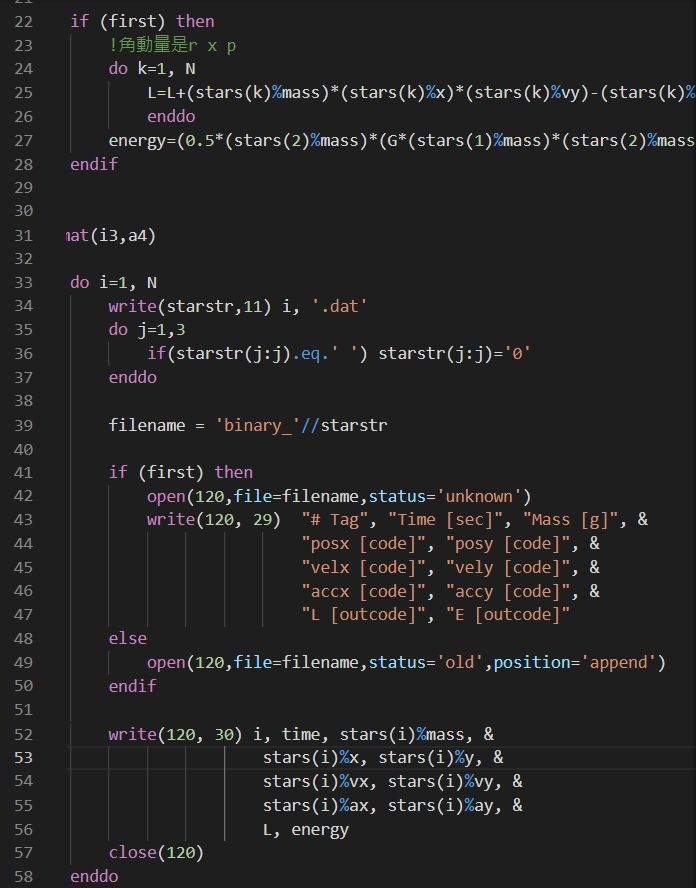
\includegraphics[scale=0.3]{pro2_cmodify.jpg}
% 	\caption{The part of modification in [output.f90].} %圖片註解
% 	\label{fig:proc_mod} %label 用這個就可以引用文章當中
% \end{figure}
% %-------------------------------

%-------------------------------
\begin{figure}[h]
    \centering
    \subfigure[dt=0.01yr]{
        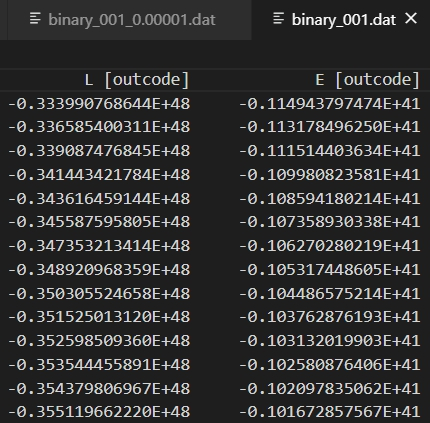
\includegraphics[scale=0.33]{01.jpg}
        \label{01}
    }
    \subfigure[dt=0.001yr]{
        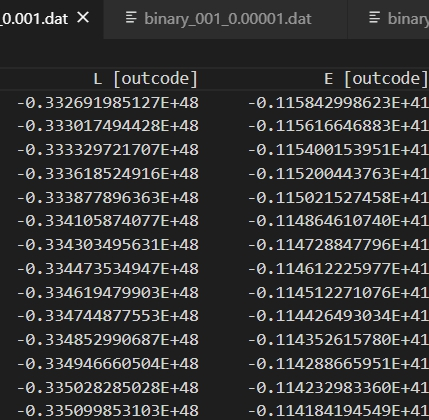
\includegraphics[scale=0.33]{001.jpg}
        \label{001} 
    }
    \subfigure[dt=0.00001yr]{
        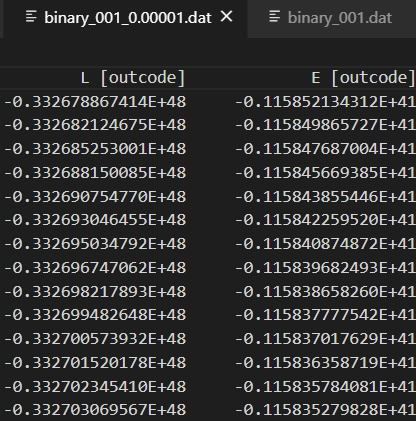
\includegraphics[scale=0.33]{00001.jpg}
        \label{00001} 
    }
    \caption{L \& E in 0.01,0.001,0.00001 time step}
    \label{fig:2c_dat}
\end{figure}

%-------------------------------
%Q3---------------------------------------------------------------------
\underline{\textbf{Q3 : Three Body problem}}\\
\textbf{3a./3b.Using ordinary/RK2 method to handle 3-body problem}

In this part, I modify the code in the update() subroutine in the [physics.f90]. The most important thing is that there are 3 body in the system, so the relations we need to consider will be $3!=6$ probabilities.

There are position $x \& y$, square of distance $rsq$, angle, force, force in x \& y direction. \textbf{All these variables need to consider 3 relations(1-2,1-3,2-3)}, not 6 because there will be 3 pairs of each variable, they will be the same value but one is positive and one is negative.

We can see that Fig.\ref{fig:3}.(a) \& (b) show the diverge result, the stars finally go away from the triple system in three different direction (coincidentally their angle seem to be $120^\circ$)
In Fig.\ref{fig:3}.(e) \& (f), the results start to converge and do \textbf{circular motion}, with a binary system inside the triple system and the other star rotation to binary system's center of mass.

I think why this system do circular motion is because : 1. this problem only consider circular obit(eccentricity=0)
2. the initial position of mass3 is far enough to let mass not suffer from too  strong gravity force which come from mass1 \& mass2.

In Fig.\ref{fig:3}.(c) \& (d) \& (g) \& (h), there are the results of RK2 method.
In program, I set the initial value of each temporary variable to become 0. We can see the reult of RK2 is a little bit converge in 0.1 \& 0.01 yr time step.(At least in Fig.\ref{fig:3}.(f) the stars rotate back to the center at the end, which is compared to  Fig.\ref{fig:3}.(b))
\\ \\
\underline{\textbf{Q4 : Solar System}}\\
In this part, I make the update() subroutine in the [physics.f90] have 2 do loops(Fig.\ref{fig:4}.(a)), the loop can repeat calculate the distance of each star (using $1<=j<=N \ \& \ 1<=k<=N$ and simultaneously $j\neq k$ )

%-------------------------------
\begin{figure}[h]
    \centering
    \subfigure[do loop]{
    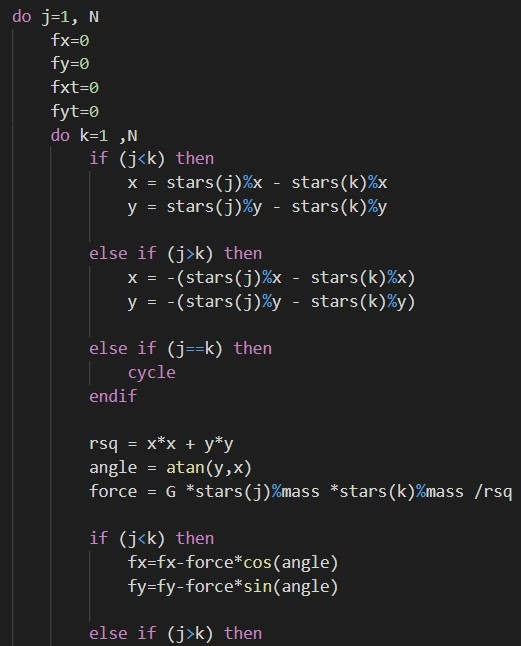
\includegraphics[scale=0.35]{program1.jpg}
    \label{program} 
    }
    \subfigure[without PLUTO]{
        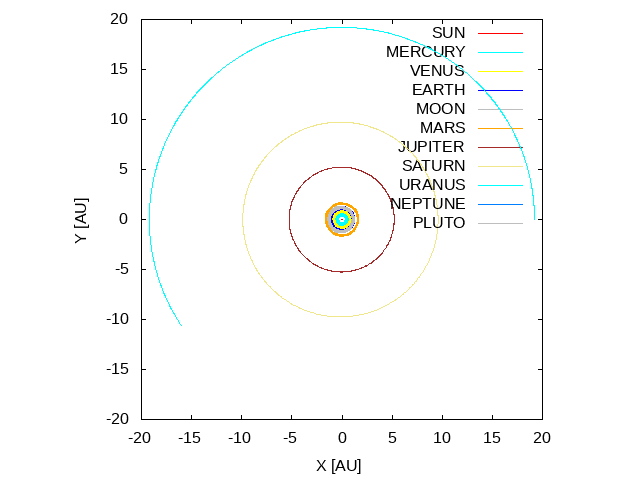
\includegraphics[scale=0.4]{pro41.png}
        \label{family}
    }
    \subfigure[terrestrial planet]{
        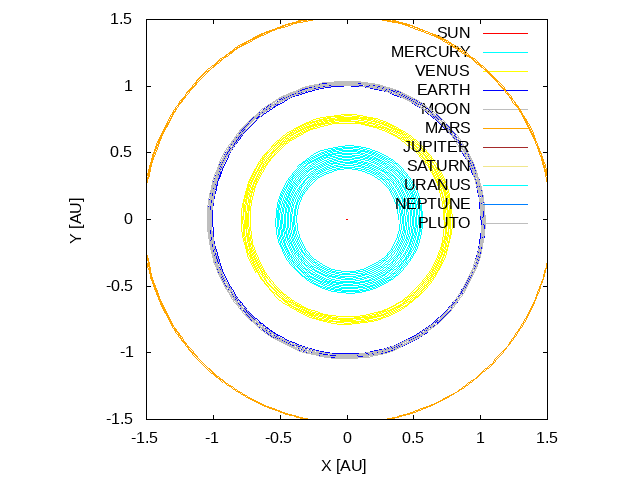
\includegraphics[scale=0.4]{pro422.png}
        \label{earth planet} 
    }
    \subfigure[Earth Moon]{
        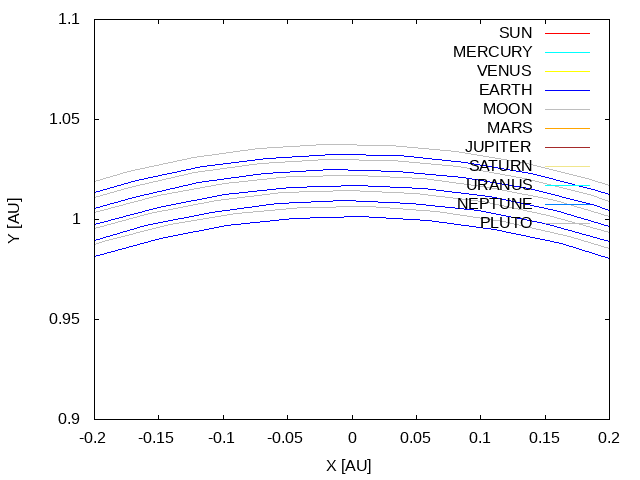
\includegraphics[scale=0.4]{pro431.png}
        \label{earth planet} 
    }
    \caption{The trajectory of solar system}
    \label{fig:4}
\end{figure}
%-------------------------------

But in this simulation, the motion of moon was false...(Fig.\ref{fig:4}.(d)). I supposed that may I neglect the velocity generated by binary system in setting the initial condition.
And MERCURY orbit become larger, I think it cause by the angular momentum lost from doing calculating (discuss in Q2.(c) the conservation of angular momentum and energy)

%-------------------------------
\begin{figure}[h]
    \centering
    \subfigure[ordinary : 0.1yr]{
        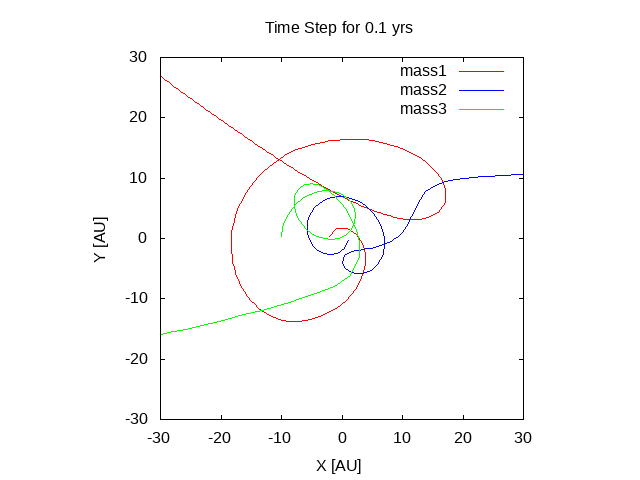
\includegraphics[scale=0.4]{pro3_a_0.1.png}
        \label{0.1}
    }
    \subfigure[ordinary : 0.01yr]{
        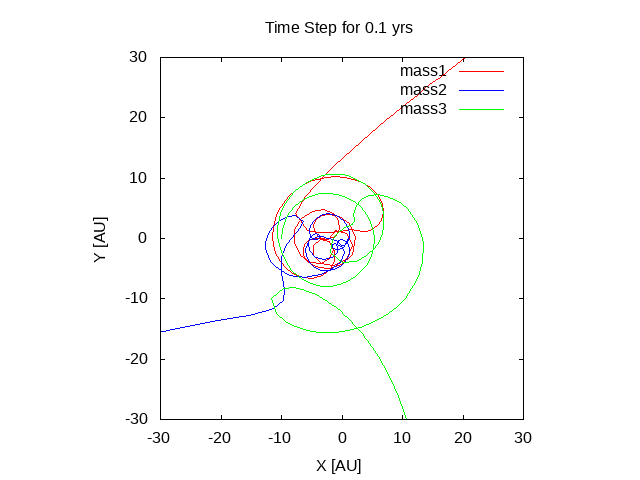
\includegraphics[scale=0.4]{pro3_a_0.01.png}
        \label{0.01} 
    }
    \subfigure[RK2 : 0.1yr]{
        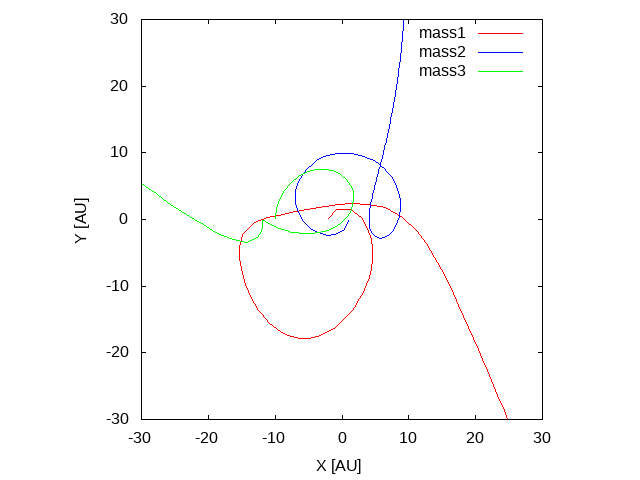
\includegraphics[scale=0.4]{pro3_b_0.1.png}
        \label{0.001} 
    }
    \subfigure[RK2 : 0.01yr]{
        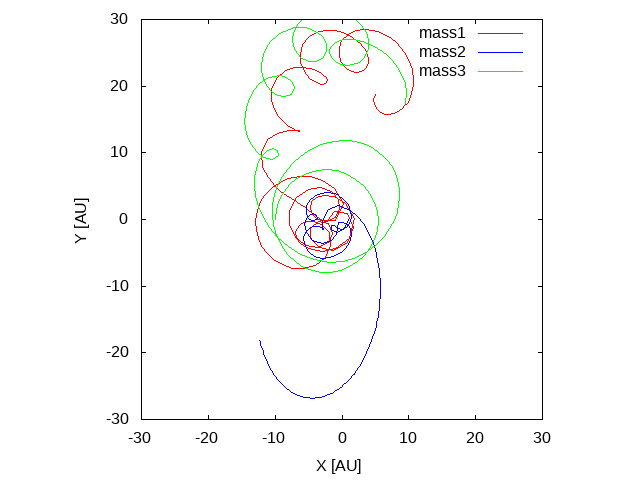
\includegraphics[scale=0.4]{pro3_b_0.01.png}
        \label{0.00001} 
    }
    \subfigure[ordinary : 0.001yr]{
        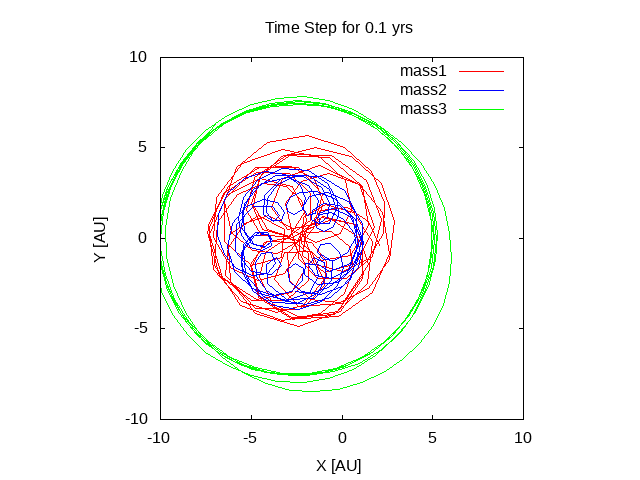
\includegraphics[scale=0.4]{pro3_a_0.001.png}
        \label{0.1}
    }
    \subfigure[ordinary : 0.00001yr]{
        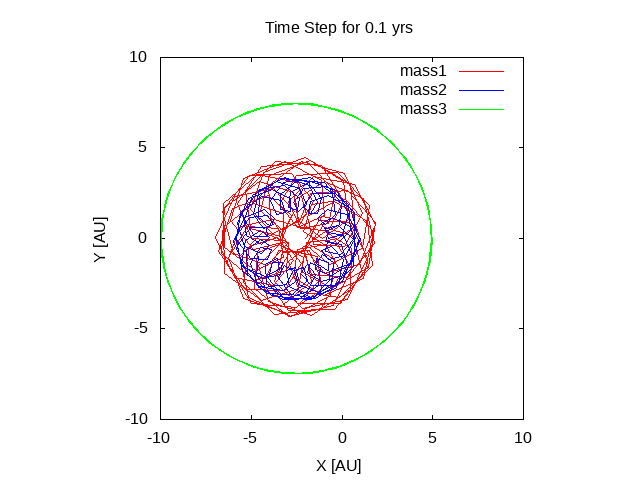
\includegraphics[scale=0.4]{pro3_a_0.00001.png}
        \label{0.01} 
    }
    \subfigure[RK2 : 0.001yr]{
        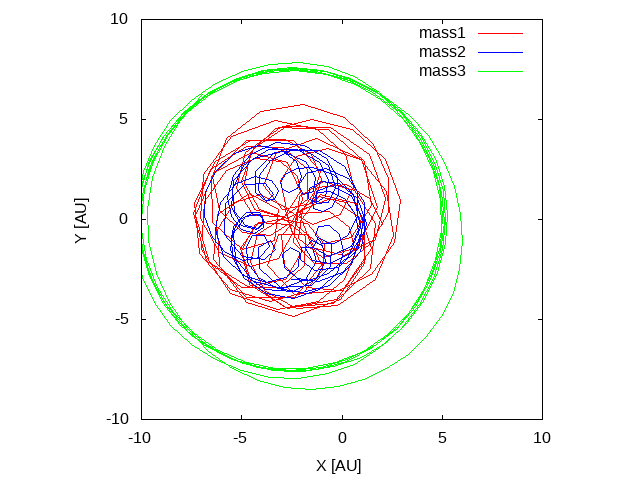
\includegraphics[scale=0.4]{pro3_b_0.001.png}
        \label{0.001} 
    }
    \subfigure[RK2 : 0.00001yr]{
        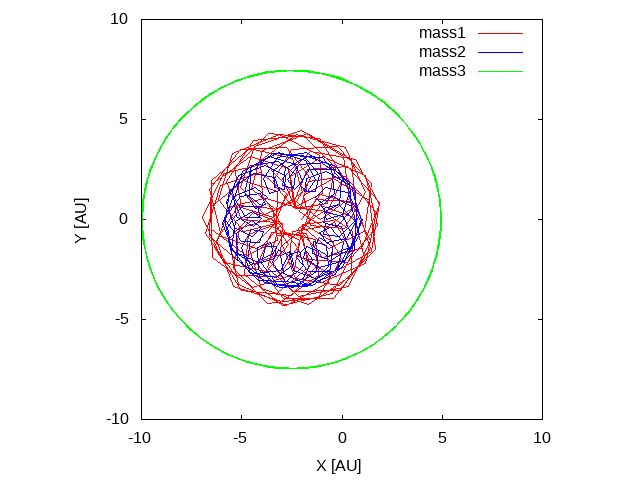
\includegraphics[scale=0.4]{pro3_b_0.00001.png}
        \label{0.00001}
    }
    \caption{Three Body simulation [ordinary method] in 0.1, 0.01, 0.001, 0.00001 yr time step\\
    .\qquad \qquad \ Three Body simulation [RK2] \qquad \qquad \quad \ in 0.1, 0.01, 0.001, 0.00001 yr time step}
    \label{fig:3}
\end{figure}

\end{document}
